\documentclass[a4paper,twocolumn]{article}

\usepackage[english]{babel}
\usepackage[utf8]{inputenc}
\usepackage{graphicx}
\usepackage{hyperref}
\usepackage{amsmath}
\usepackage{fullpage}
\usepackage{titlesec}

\titleformat*{\section}{\large\bfseries}
\titleformat*{\subsection}{\normalsize\bfseries}
\let\originalleft\left
\let\originalright\right
\renewcommand{\left}{\mathopen{}\mathclose\bgroup\originalleft}
\renewcommand{\right}{\aftergroup\egroup\originalright}

\title{Learning without Forgetting $-$ summary}
\author{Matěj Nikl}

\begin{document}
\maketitle
This paper is about a method called Learning without Forgetting (LwF), which focuses on the task of incremental learning of new capabilities without forgetting the old ones. On top of that, this method can accomplish this task without the need for the training data the old capabilities were trained with.

It resembles the combination of \textit{Knowledge Distilling} and transfer learning strategy \textit{fine-tuning}.

\section{The Architecture}
The LwF's view on a model consists of:
\begin{itemize}
    \item shared parameters $\theta_s$
    \item task-specific parameters for previously learned tasks $\theta_o$
    \item randomly initialized task-specific parameters for new tasks $\theta_n$
\end{itemize}
It is useful to think of $\theta_o$ and $\theta_n$ as classifiers (fully connected layers) that operate on features parameterized by $\theta_s$ (see Figure \ref{fig:methods})

\section{Learning without Forgetting}
Given a (C)NN with $\theta_s$ and $\theta_o$, the goal is to add $\theta_n$ for new tasks and learn all the parameters that work well on both old and new tasks, using only labeled data for the new tasks:
\begin{enumerate}
    \item record responses (probability distributions over classes) $y_o$ for each example of the new dataset from the original network (defined by $\theta_s$ and $\theta_o$)
    \item add new fully connected classifiers $\theta_n$ on top of $\theta_s$, that will compute the new tasks' class probability distributions
    \item fine-tune $\theta_n$ using supervised cross-entropy loss \ref{ssec:CEloss} (sum over losses if multiple new tasks) until convergence (having $\theta_s$ (and $\theta_o$) frozen)
    \item train all parameters jointly using a (weighted) sum of supervised cross-entropy loss and Knowledge Distillation loss \ref{ssec:KDloss} (sum over losses if multiple old tasks) until convergence
\end{enumerate}

\subsection{Cross-entropy loss}
\label{ssec:CEloss}
\begin{equation*}
    \mathcal{L}_{\mathrm{new}}(y_n, \hat{y}_n) = -y_n \log\hat{y}_n
\end{equation*}

\subsection{Knowledge Distillation loss}
\label{ssec:KDloss}
The Knowledge Distillation loss adds the objective of keeping the outputs of the old task classifiers for all of the new dataset inputs the same as they were, before the learning of the new tasks began.
\begin{align*}
    \mathcal{L}_{\mathrm{old}}(y_o, \hat{y}_o) &= D_{\mathrm{KL}}(y_o^\prime\|\hat{y}_o^\prime) \\
                &= - \sum_{i=1}^l y_o^{\prime(i)} \log(\hat{y}_o^{\prime(i)}) \\
                &= - \sum_{i=1}^l \left( \frac{e^{y_o^{(i)}/T}}{\sum_j e^{y_o^{(j)}/T}} \log \left( \frac{e^{\hat{y}_o^{(i)}/T}}{\sum_j e^{\hat{y}_o^{(j)}/T}} \right) \right)
\end{align*}
where $l$ is the number of classes and $T$ is the temperature of the softmax function. The recommended setting is $T > 1$, because then the weight of smaller logit is bigger and encourages the network to better encode similarities among classes. % The used setting in this paper was $T = 2$.

\section{Principles of modularization}
Each of the $\theta_o$ output classifiers can be seen as a module. There is no need for the network to always output all $\theta_o$ outputs $-$ only a selected output classifier for the selected task at hand can be connected to produce the desired output. The output classifiers, however, ale strongly tied to the shared parameters $\theta_s$ with whom they have been trained with. The output modules are thus not transferable to a different model with different $\theta_s$.

\section{Principles of growing}
For each new task a new output layer $\theta_n$ is crated. The whole set of parameters $\theta$ is adjusted:
\begin{itemize}
    \item $\theta_s$ and $\theta_o$ in such a way that they allow for the new task to be learned, while also retaining the old knowledge
    \item $\theta_n$ in such a way that it performs well on the new task
\end{itemize}


\begin{figure*}[t]
    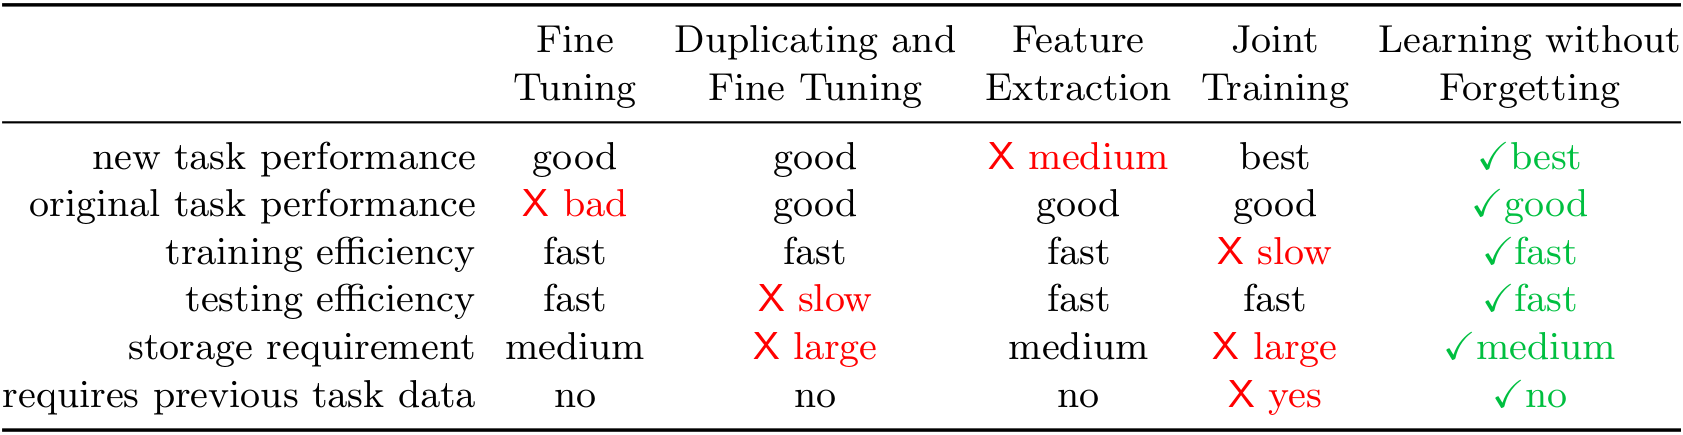
\includegraphics[width=\textwidth]{table.png}
    \caption{Relative advantages of the LwF method compared to other commonly used methods.}
    \label{fig:table}
\end{figure*}
\begin{figure*}[t]
    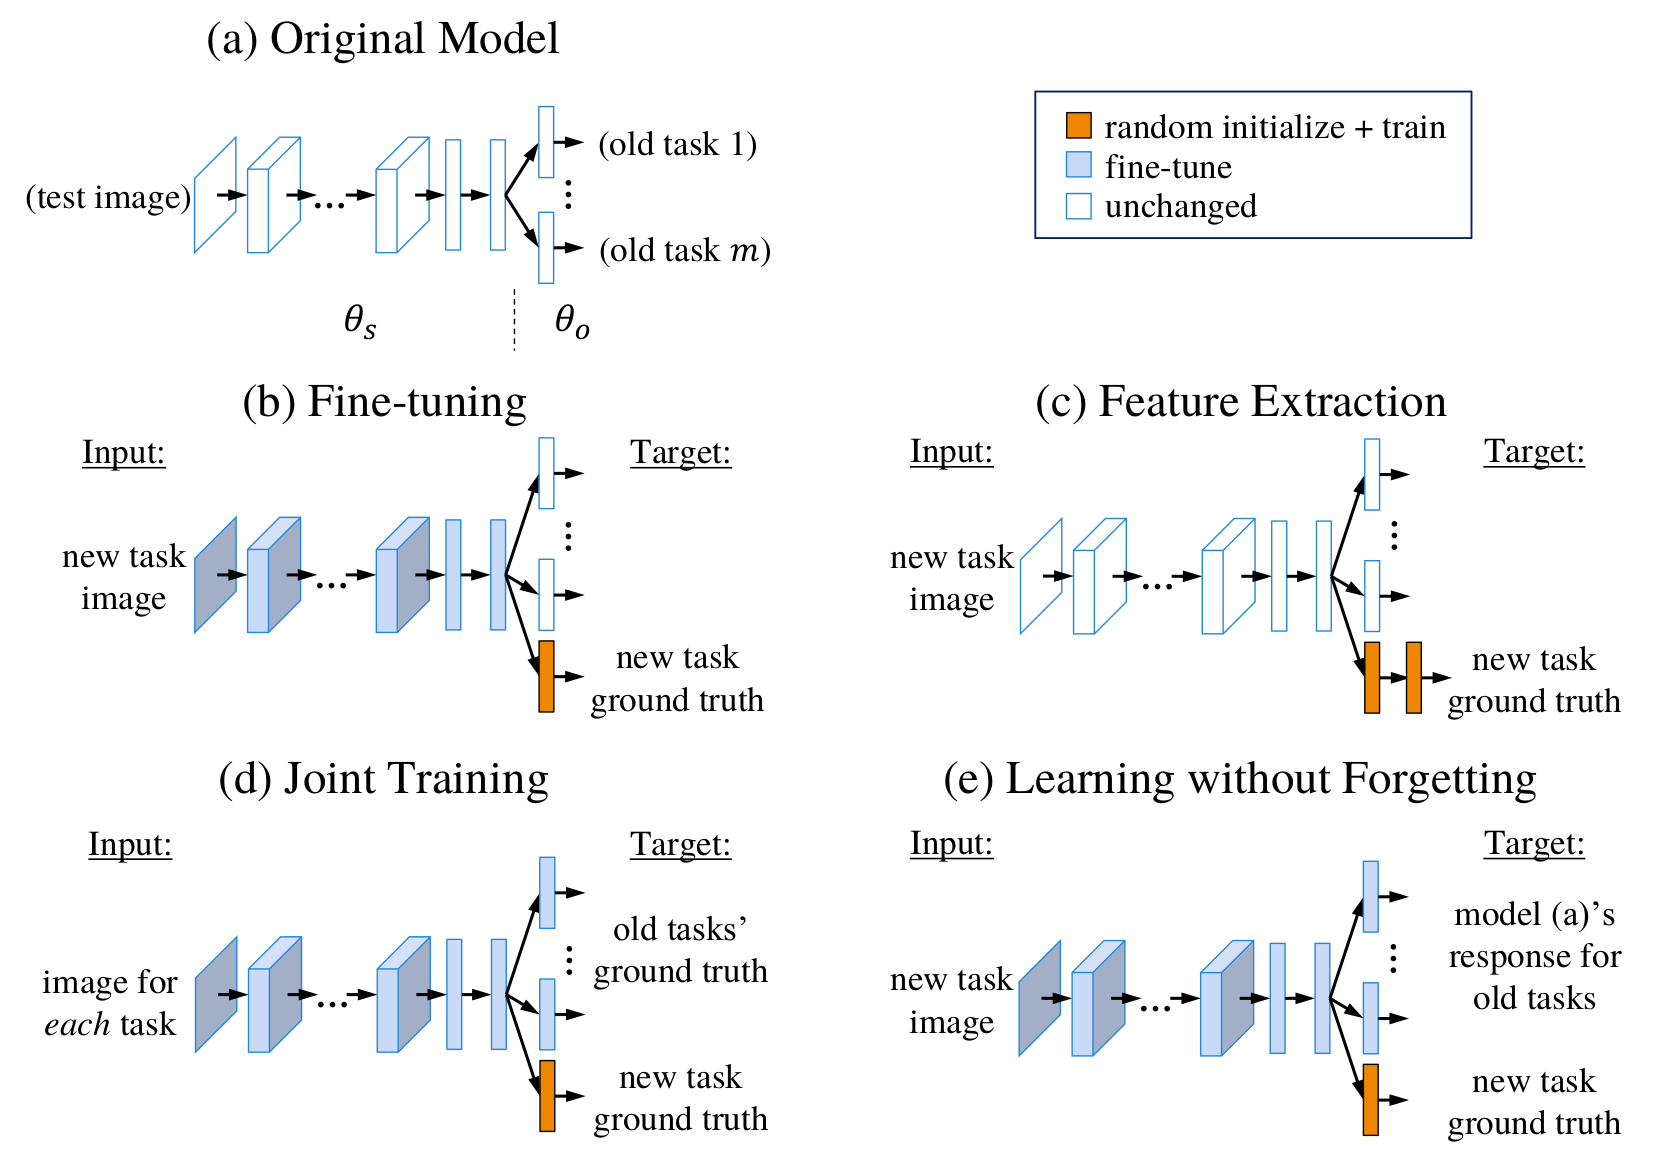
\includegraphics[width=\textwidth]{methods.png}
    \caption{Illustration of LwF method (e) and other methods (b-d).}
    \label{fig:methods}
\end{figure*}
\end{document}
